This section shows the screenshot of the web interface used in the user evaluation study (see Section~\ref{subsubsec:quantitative_analysis_of_user_ratings} for the explanation flow).

\vspace{-0.5em}

\begin{figure}[h]
    \centering
    \captionsetup{font=small,skip=4pt}
    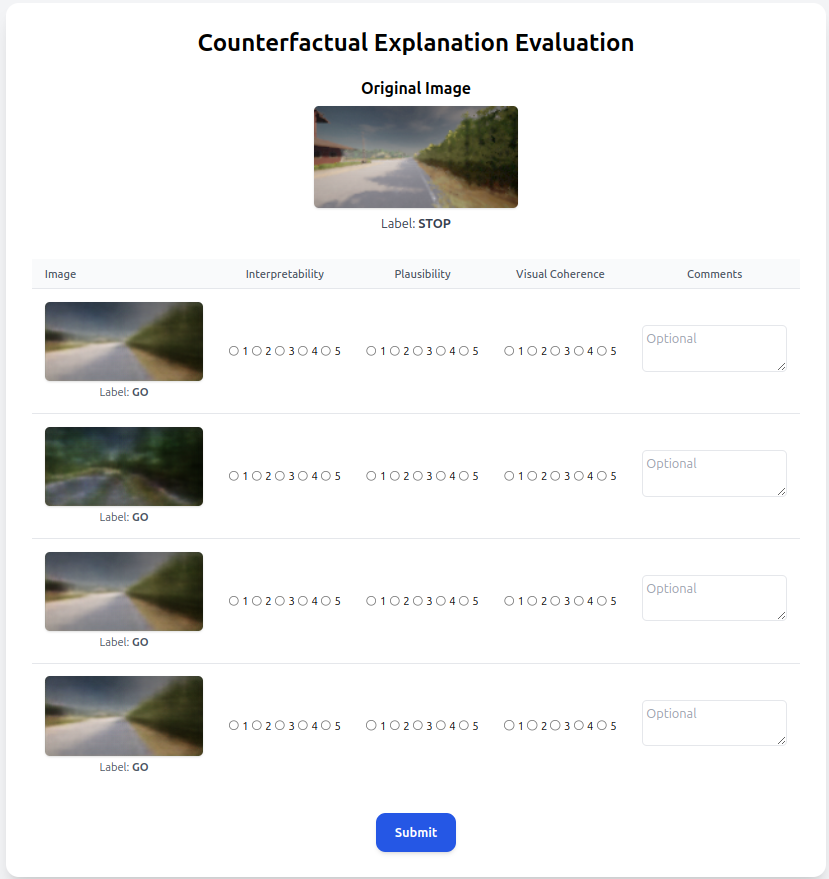
\includegraphics[width=0.68\textwidth]{img/web_app_screenshots/grading.png}
    \caption[Web interface: counterfactual rating task]{%
Screenshot of the web-based evaluation interface used in the human user study. The top shows the original driving scene (predicted as \texttt{STOP}), followed by four counterfactuals (e.g., predicted as \texttt{GO}). Participants rated each on interpretability, plausibility, and visual coherence using a 5-point Likert scale. Optional textboxes allowed for qualitative comments. The full setup is discussed in Section~\ref{subsubsec:quantitative_analysis_of_user_ratings}.}
    \label{fig:app:grading}
\end{figure}


\begin{sidewaysfigure}[htbp]
    \centering
    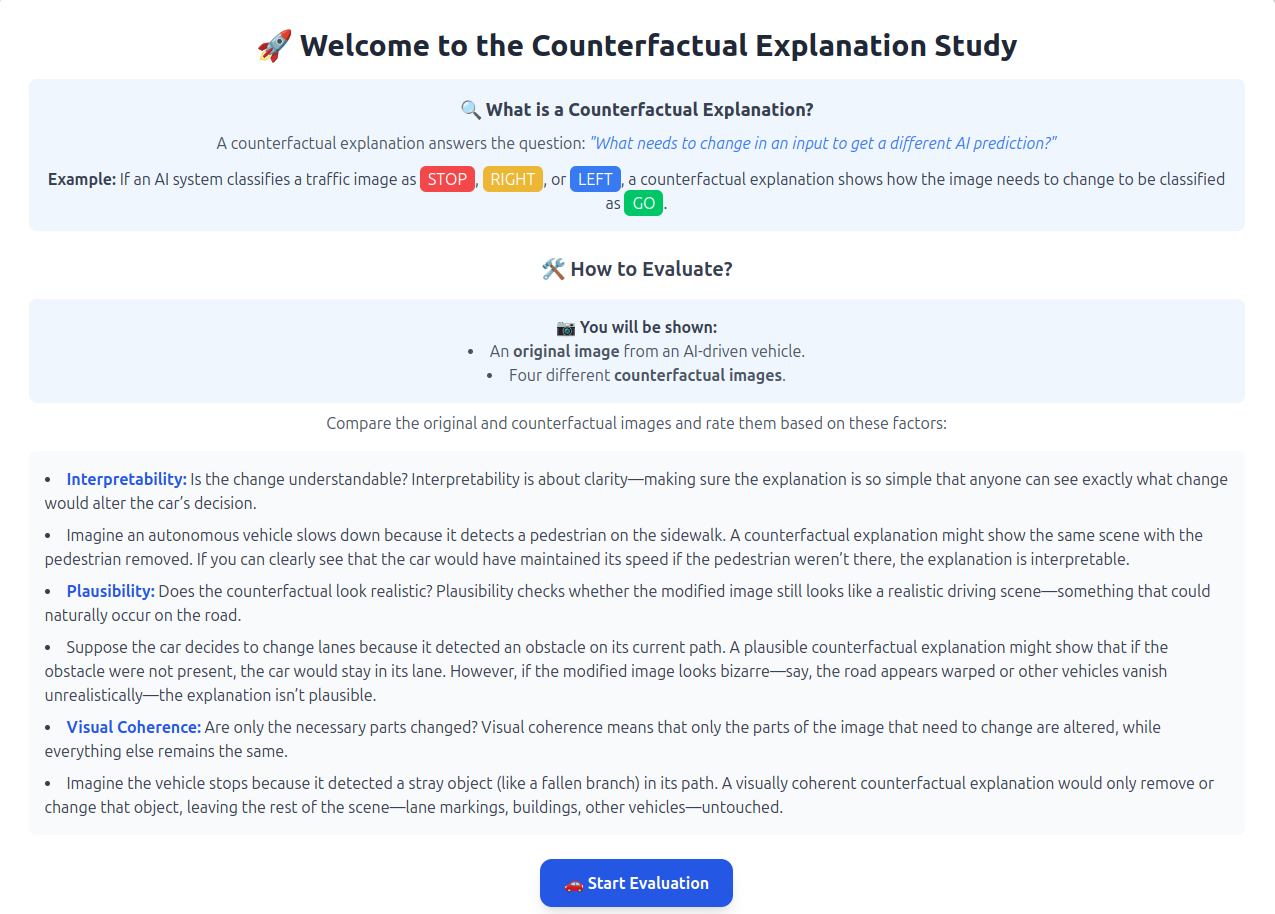
\includegraphics[width=0.78\textwidth]{img/web_app_screenshots/form_ui_info.png}
    \caption[Welcome screen of user study interface]{%
Welcome screen of the user evaluation interface for the counterfactual explanation study. It introduces the purpose of the task—evaluating counterfactual examples classification—and describes what participants will see and how to evaluate each explanation based on three criteria: interpretability, plausibility, and visual coherence. Definitions and examples are included to ensure consistent understanding.}
    \label{fig:app:form_ui}
\end{sidewaysfigure}